\documentclass[12pt]{article}

\usepackage[T1]{fontenc}
\usepackage[utf8]{inputenc}
\usepackage[russian]{babel}

\usepackage{amsmath}
\usepackage{float}
\usepackage{tabularx}

\usepackage{textcomp}

% page margin
\usepackage[top=2cm, bottom=2cm, left=2cm, right=2cm]{geometry}

\usepackage{graphicx}

\usepackage{fancyhdr}
\pagestyle{fancy}
% modifying page layout using fancyhdr
\fancyhf{}
\renewcommand{\sectionmark}[1]{\markright{\thesection\ #1}}
\renewcommand{\subsectionmark}[1]{\markright{\thesubsection\ #1}}

\rhead{\fancyplain{}{\rightmark }}
\cfoot{\fancyplain{}{\thepage }}

\renewcommand{\arraystretch}{1.3}

\begin{document}

\vspace*{-2cm}
\begin{figure}[!ht]
	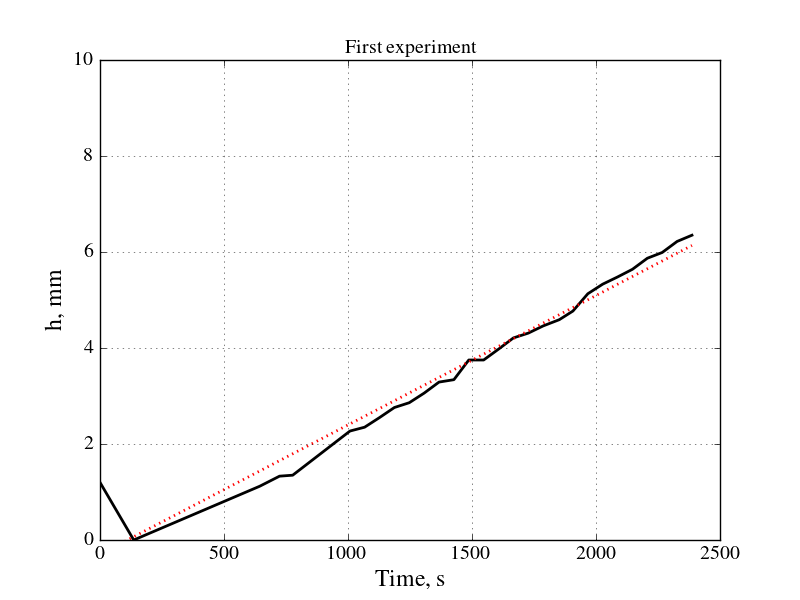
\includegraphics[width = 0.33\linewidth]{../1exp_new.png}
	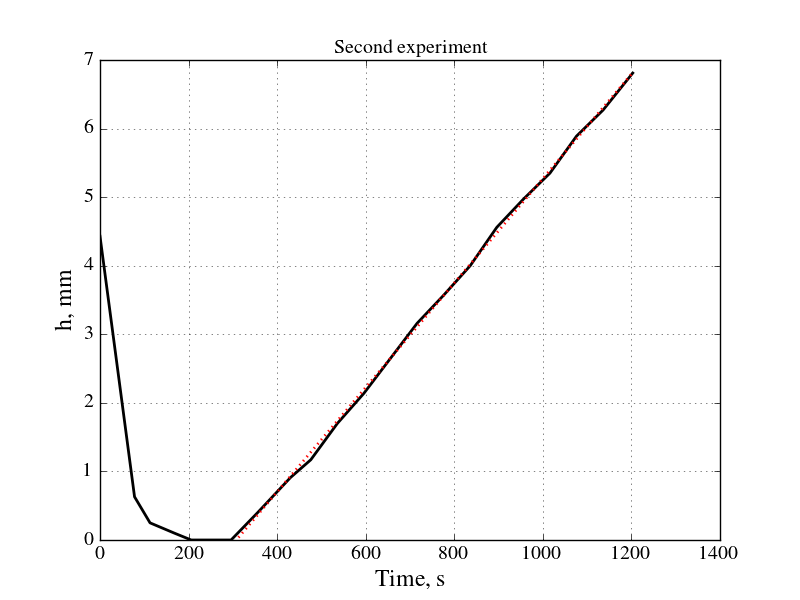
\includegraphics[width = 0.33\linewidth]{../2exp_new.png}
	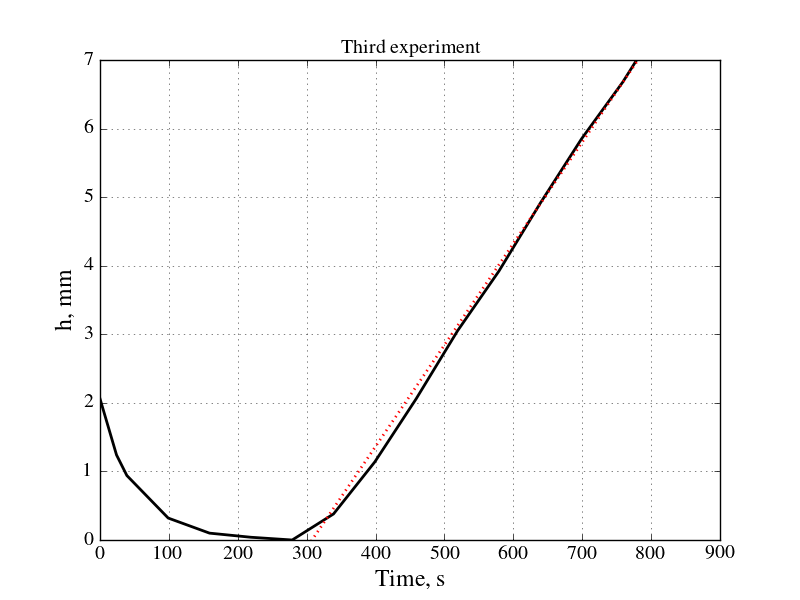
\includegraphics[width = 0.33\linewidth]{../3exp_new.png}
	\caption{Зависимости положения мениска от времени в трех экспериментах}
\end{figure}

\begin{table}[!ht]
\begin{center}
\caption{Концентрации компонентов в исследуемых растворах}
\begin{tabular}{>{\centering}m{2cm} >{\centering}m{1.2cm} >{\centering}m{1.2cm} >{\centering}m{1.2cm} m{1.2cm}}
	\hline
	& $\mathbf{A}$, мл & $\mathbf{B}$, мл & $\mathbf{C}$, мл & {\centering}$\mathbf{D}$, мл \\
	I состав & 1 & 8 & 1 & {\centering}-\\
	II состав & 3 & 6 & 1 & {\centering}-\\
	III состав & 7 & 2 & - & {\centering}1 \\
	\hline
\end{tabular}
\end{center}
\end{table}

$\mathbf{A}$ -- раствор инициатора в ММА ($0.01$ г/мл); $\mathbf{B}$ -- раствор иницатора в бензоле ($0.01$ г/мл); $\mathbf{C}$ --чистый ММА; $\mathbf{D}$ -- раствор TEMPO в МMA ($1.5 \cdot 10^{-3}$ M).

Скорость полимеризации $V_r$ рассчитывалась по формуле
\begin{gather}
 	-\frac{d \left[ M \right]}{dt} = V_r = \frac{\pi r^2}{V_0 \, \delta_M M} \frac{\Delta h}{\Delta t}, \notag
\end{gather}  
где $\delta_M$ -- параметр контракции -- является разностью обратных плотностей мономера и полимера
\begin{gather}
	\delta_M = \frac{1}{\rho_M} - \frac{1}{\rho_\textup{П}}, \notag
\end{gather}

а объем при температуре $T = 70^{\circ}C$ пересчитывался через объем при комнатной температуре при помощи коэффициента термического расширения $\alpha$:
\begin{gather}
	V_0 = V_0^{\prime} \left( 1 + \alpha \cdot \left( 70 - 20 \right) \right) \notag
\end{gather}

\begin{table}[!ht]
\begin{center}
\caption{}
\begin{tabular}{ccccc}
	\hline
	Номер эксперимента & [M], моль/л & log [M] & v$_p$, моль/л$\cdot$с & log v$_p$ \\
	%\hline
	\#1 & 1.872 & 0.627 & 1.18$\cdot 10^{-4}$ & -9.05 \\
	\#2 & 3.744 & 1.320 & 3.35$\cdot 10^{-4}$ & -8.00 \\
	\#3 & 7.488 & 2.013 & 6.50$\cdot 10^{-4}$ & -7.34 \\  
	\hline
\end{tabular}
\end{center}
\end{table}

\begin{figure}[!ht]
	\centering
	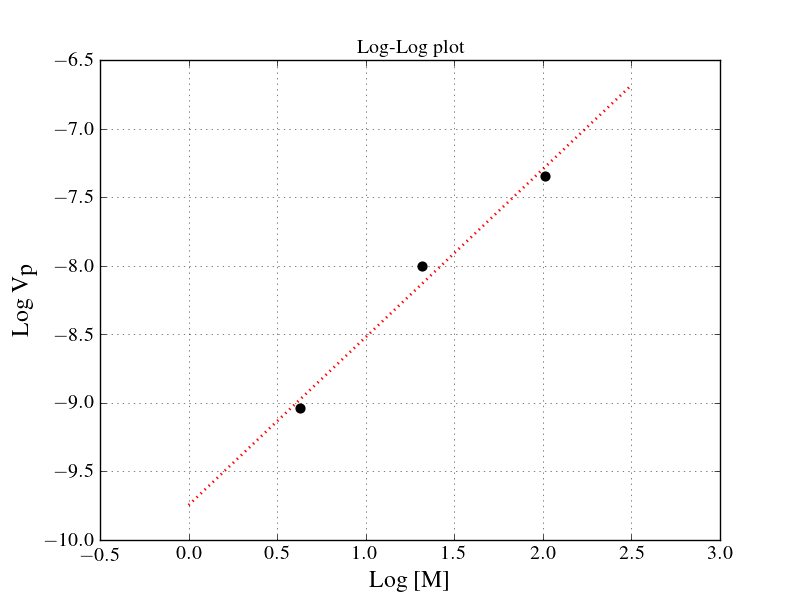
\includegraphics[width = 0.7\linewidth]{../loglog.png}
	\caption{Определение порядка реакции по инициатору}
\end{figure}

Порядок реакции по ММА 1.23.

Определим скорость ингибирования по формуле
\begin{gather}
		v_{inh} = \frac{[TEMPO]}{t_{inh}}, \quad t_{inh} = t_2 - t_3, \notag
\end{gather}
где $t_2$, $t_3$ -- времена, отсекаемые прямыми на центральном и правом графиках на рис. 1, а $[TEMPO]$ -- концентрация TEMPO в реакционной смеси ( 1.5$\cdot 10^{-4}$M ). Скорость ингибирования $v_{inh} = 8.24 \cdot 10^{-5} M/s$. \par
Определим константу распада по следующей формуле
\begin{gather}
	k_{dis} = \frac{v_{inh}}{2 \cdot f \cdot [I]} = 4.97 \cdot 10^{-3} s^{-1}, \quad f \approx 0.5 \notag
\end{gather}

Длину кинетической цепи $Y_{kin}$ определяют в условиях квазистационарности радикалов из соотношения скоростей роста цепи и ингибирования:
\begin{gather}
		Y_{kin} = \frac{v_p}{v_{inh}} = 4.075 \notag
\end{gather}

\section{Вопросы}
\begin{enumerate}
	\item На чем основано определение скорости инициирования? \\
	Метод определения скорости инициирования основан на измерении скорости полимеризации при разных концентрациях инициатора на начальных конверсиях мономера.
	\item В чем отличие константы инициирования от константы распада инициатора? \\
	Константа распада инициатора определяет распад инициатора с образованием радикалов, которые инициируют процесс радикальной полимеризации мономеров. Инициация мономеров определяется константой инициирования. Константа инициирования связана с константой распада инициатора эффективностью инициатора.
	\item Какую информацию дает величина длины кинетической цепи? \\
	Кинетическая цепь -- число молекул мономера, приходящихся на один образовавшийся радикал $R\cdot$  до его гибели при обрыве цепи. Эта величина напрямую связана со среднечисловой степенью полимеризации ( в зависимости от преобладающего типа обрыва цепи, они связаны по-разному). 
\end{enumerate}


\end{document}
